% Options for packages loaded elsewhere
\PassOptionsToPackage{unicode}{hyperref}
\PassOptionsToPackage{hyphens}{url}
%
\documentclass[
]{article}
\usepackage{amsmath,amssymb}
\usepackage{iftex}
\ifPDFTeX
  \usepackage[T1]{fontenc}
  \usepackage[utf8]{inputenc}
  \usepackage{textcomp} % provide euro and other symbols
\else % if luatex or xetex
  \usepackage{unicode-math} % this also loads fontspec
  \defaultfontfeatures{Scale=MatchLowercase}
  \defaultfontfeatures[\rmfamily]{Ligatures=TeX,Scale=1}
\fi
\usepackage{lmodern}
\ifPDFTeX\else
  % xetex/luatex font selection
\fi
% Use upquote if available, for straight quotes in verbatim environments
\IfFileExists{upquote.sty}{\usepackage{upquote}}{}
\IfFileExists{microtype.sty}{% use microtype if available
  \usepackage[]{microtype}
  \UseMicrotypeSet[protrusion]{basicmath} % disable protrusion for tt fonts
}{}
\makeatletter
\@ifundefined{KOMAClassName}{% if non-KOMA class
  \IfFileExists{parskip.sty}{%
    \usepackage{parskip}
  }{% else
    \setlength{\parindent}{0pt}
    \setlength{\parskip}{6pt plus 2pt minus 1pt}}
}{% if KOMA class
  \KOMAoptions{parskip=half}}
\makeatother
\usepackage{xcolor}
\usepackage{graphicx}
\makeatletter
\def\maxwidth{\ifdim\Gin@nat@width>\linewidth\linewidth\else\Gin@nat@width\fi}
\def\maxheight{\ifdim\Gin@nat@height>\textheight\textheight\else\Gin@nat@height\fi}
\makeatother
% Scale images if necessary, so that they will not overflow the page
% margins by default, and it is still possible to overwrite the defaults
% using explicit options in \includegraphics[width, height, ...]{}
\setkeys{Gin}{width=\maxwidth,height=\maxheight,keepaspectratio}
% Set default figure placement to htbp
\makeatletter
\def\fps@figure{htbp}
\makeatother
\setlength{\emergencystretch}{3em} % prevent overfull lines
\providecommand{\tightlist}{%
  \setlength{\itemsep}{0pt}\setlength{\parskip}{0pt}}
\setcounter{secnumdepth}{-\maxdimen} % remove section numbering
\ifLuaTeX
  \usepackage{selnolig}  % disable illegal ligatures
\fi
\IfFileExists{bookmark.sty}{\usepackage{bookmark}}{\usepackage{hyperref}}
\IfFileExists{xurl.sty}{\usepackage{xurl}}{} % add URL line breaks if available
\urlstyle{same}
\hypersetup{
  pdftitle={CalcNum-merged},
  hidelinks,
  pdfcreator={LaTeX via pandoc}}

\title{CalcNum-merged}
\author{}
\date{}

\begin{document}
\maketitle

\hypertarget{introduzione}{%
\section{0. Introduzione}\label{introduzione}}

Branca della matematica che si occupa di dare strumenti per il calcolo
numerico di quantità continue (soluzioni di
un\textquotesingle equazione)

Example

{} soluzione {}

{} (soluzione simbolica)

{} limite dell\textquotesingle iterazione

{}

\hypertarget{calcolo-simbolico-vs-calcolo-numerico}{%
\section{Calcolo Simbolico VS Calcolo
Numerico}\label{calcolo-simbolico-vs-calcolo-numerico}}

Example

{} con {} ha un\textquotesingle unica soluzione {}

\begin{itemize}
\tightlist
\item
  {} soluzione simbolica
\item
  {} è il limite dell\textquotesingle iterazione:{}
\end{itemize}

Example

Eq: {} unica soluzione {}

\begin{itemize}
\tightlist
\item
  {} non esprimibile in forma chiusa con simboli noti (soluzione
  simbolica)
\item
  {} è il limite dell\textquotesingle iterazione:{}
\end{itemize}

Quasi tutte le civiltà hanno una formula per le equazioni di 2° grado.

Nel XVI secolo sono state trovate per le equazioni di 3° e 4° grado
(Tartaglia, Cardano, Ferrari).

Important

Teorema di Ruffini-Abel:

Non esiste una formula per le equazioni di 5° grado

La materia si occupa di dare strumenti teorici (teorie matematiche) per
il calcolo numerico di quantità continue.

Si cerca di trovare una soluzione ai problemi continui che sia
utilizzabile. Non basta una formula, ma serve un algoritmo che fornisca
una soluzione in un tempo ragionevole tenendo conto che il calcolatore
lavora in quantità finite. Vogliamo quindi trattare \textbf{quantità
infinite} con \textbf{strumenti finiti}.

\hypertarget{quantituxe0-continue}{%
\section{Quantità Continue}\label{quantituxe0-continue}}

\begin{itemize}
\tightlist
\item
  Una o più equazioni non lineari, radici di polinomi
\item
  Calcolo quantità algebra lineare, soluzione di sistemi lineari
\item
  Determinanti, autovalori/vettori, rango, nucleo, immagine
\item
  Calcolo degli integrali
\item
  Approssimazione di funzioni
\end{itemize}

Per ogni problema esistono una o più soluzioni.

\hypertarget{efficienza}{%
\subsection{Efficienza}\label{efficienza}}

Gli algoritmi devono avere importanti requisiti:

\begin{itemize}
\tightlist
\item
  Basso costo computazionale
\item
  Stabilità numerica
\end{itemize}

\hypertarget{stabilituxe0-numerica}{%
\section{1. Stabilità numerica}\label{stabilituxe0-numerica}}

Esempio

\hypertarget{sviluppo-in-serie-di-taylor-di-con-resto-di-lagrange}{%
\subsection{\texorpdfstring{Sviluppo in serie di Taylor di {} con resto
di
Lagrange}{Sviluppo in serie di Taylor di  con resto di Lagrange}}\label{sviluppo-in-serie-di-taylor-di-con-resto-di-lagrange}}

{}

Si hanno due algoritmi per il calcolo di {}\\
{}{}

Il primo funziona meglio con esponente positivo, il secondo con
esponente negativo

\hypertarget{relazioni-con-altre-discipline}{%
\section{Relazioni Con Altre
Discipline}\label{relazioni-con-altre-discipline}}

\hypertarget{matematica-discreta}{%
\subsection{Matematica Discreta}\label{matematica-discreta}}

Si cerca di utilizzare una sola formula per la risoluzione di problemi,
mentre qua ci servono più formule

\hypertarget{algoritmi-e-strutture-dati}{%
\section{Algoritmi E Strutture Dati}\label{algoritmi-e-strutture-dati}}

Si occupa dello studio di problemi discreti, mentre qui ci si occupa di
problemi continui

\hypertarget{relazione-con-il-mondo-reale}{%
\section{Relazione Con Il Mondo
Reale}\label{relazione-con-il-mondo-reale}}

I problemi del mondo reale possono essere \textbf{modellizzati} in
teorie matematiche.

Le soluzioni matematiche vengono \textbf{applicate} nel mondo reale.

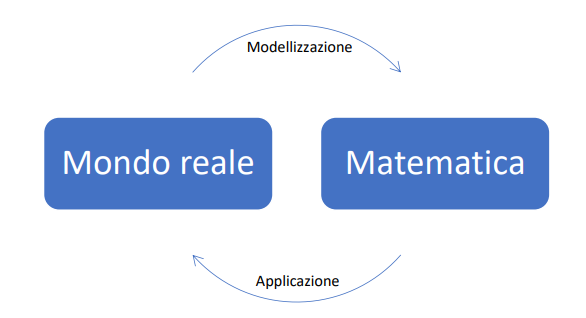
\includegraphics{/home/michi/Documenti/Uni/Modellizzazione.png}

\hypertarget{error-analysis}{%
\section{2. Error Analysis}\label{error-analysis}}

I numeri reali per la maggior parte contengono infinite informazioni, a
parte i pochi numeri razionali che ne contengono di limitate.

\hypertarget{numeri-razionali}{%
\section{Numeri Razionali}\label{numeri-razionali}}

Sono dei numeri che rispettano la descrizione di un determinato teorema,
e che non rispettano altri teoremi come, ad esempio, il teorema degli
zeri o quello di Lagrange.

I numeri razionali sono infiniti, ma noi possiamo lavorare solo con
insiemi finiti di numeri.

Problema

Selezionare un numero finito di valori che possano rappresentare i
numeri reali.

\hypertarget{distribuzione-uniforme}{%
\subsection{Distribuzione uniforme}\label{distribuzione-uniforme}}

Scegliere {}, N pari:\\
{}

Possiamo rappresentare i numeri reali con l\textquotesingle insieme:

\hypertarget{errore-assoluto-vs-relativo}{%
\section{Errore Assoluto Vs
Relativo}\label{errore-assoluto-vs-relativo}}

\begin{itemize}
\tightlist
\item
  Errore assoluto: {}
\item
  Errore relativo: {}
\end{itemize}

\hypertarget{problemi-con-lerrore-assoluto}{%
\subsection{Problemi Con L\textquotesingle errore
Assoluto}\label{problemi-con-lerrore-assoluto}}

La qualità dell\textquotesingle approssimazione
dell\textquotesingle errore assoluto non è sempre la stessa, ad esempio
per i numeri più piccoli c\textquotesingle è un errore più grande
rispetto a quelli più grandi.

Con l\textquotesingle errore relativo le cifre errate nella
rappresentazione dei numeri sono sempre le stesse.

A noi serve sapere solo alcune cifre, quindi è meglio utilizzare una
rappresentazione dei numeri con l\textquotesingle errore relativo
migliore.

\hypertarget{numeri-reali}{%
\section{Numeri Reali}\label{numeri-reali}}

Limiti di sequenze di numeri razionali che possono essere approssimate.

Data una base di numerazione {} posso prendere un numero reale tra 0 e 1
e le sequenze di cifre

{}

Teorema Della Rappresentazione In Basi

Dato {} e data una base di numerazione {} esiste un unico {} e una
sequenza {} tali che:

\begin{enumerate}
\tightlist
\item
  {}
\item
  {}
\item
  {} non è definitivamente uguale a {} così che {}
\end{enumerate}

Il numero {} si dice \textbf{mantissa}

\hypertarget{floating-point}{%
\subsection{Floating Point}\label{floating-point}}

Data una base di numerazione {}, il numero {} di cifre della mantissa
{}, {} numeri positivi, definiamo un insieme di \textbf{floating point
numbers}

{}{}

Esempio

{}

Cardinalità: {}

Max(F): {}

MinPositivo(F): {}

Per {} i numeri non possono essere rappresentati, mentre per {}
c\textquotesingle è un grande errore relativo

Esempio 2 (Utile per dopo)

{} è composto da 13 numeri

Questi numeri \textbf{non sono uniformi}. Tra {} e {} e tra {} e 1
c\textquotesingle è lo stesso numero di elementi di {}.

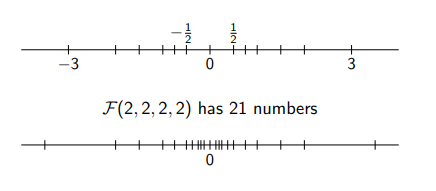
\includegraphics{/home/michi/Documenti/Uni/Pasted image 20230125111411.png}

Data {} costruiamo una \textbf{funzione di rappresentazione}\\
{}

Con una delle due regole, dato {}:

\begin{itemize}
\tightlist
\item
  Troncamento: {}
\item
  Arrotondamento: {} il troncamento di {}
\end{itemize}

Se {} impostiamo {} (\textbf{overflow}), se {} impostiamo {}
(\textbf{underflow}), stesso ragionamento per i numeri negativi.

Definiamo la \textbf{precisione macchina} come {} per il troncamento e
{} per l\textquotesingle arrotondamento.

Teorema

Dato {} abbiamo il seguente limite per l\textquotesingle errore
relativo:\\
{}

\textbf{{} deve seguire determinate proprietà algebriche}:

{}

Dobbiamo definire delle \textbf{operazioni} con i numeri a virgola
mobile.

Assumendo che esiste una somma a virgola mobile {} tale che se {} (se
non avviene overflow):

{}

Similmente definiamo {}.

Un\textquotesingle idea è quella di definire {} ma i dettagli sono più
complicati.

Infatti le varie operazioni seguono solo alcune delle proprietà delle
operazioni elementari:

\begin{itemize}
\tightlist
\item
  commutatività della somma
\item
  commutatività del prodotto
\item
  {}
\end{itemize}

Non seguono infatti:

\begin{itemize}
\tightlist
\item
  associatività di somma e prodotto
\item
  proprietà distributiva
\item
  semplificazione
\item
  potrebbe succedere che {}
\end{itemize}

3. Errore Per Le Funzioni Razionali

\hypertarget{errore-per-le-funzioni-razionali}{%
\section{3. Errore Per Le Funzioni
Razionali}\label{errore-per-le-funzioni-razionali}}

Data una funzione razionale {} che sia {} con {} e {} polinomi.

Dall\textquotesingle analisi matematica sappiamo che {} è definita e
differenziabile per {} (assumendo che {} e {} siano primi).

Ci sono due tipi di errori nella valutazione di {} con i valori in
virgola mobile

\hypertarget{errore-inerente}{%
\subsection{Errore Inerente}\label{errore-inerente}}

Non valutiamo {} ma valutiamo {} dove {} funzione approssimata

{}

Se l\textquotesingle errore inerente è relativamente piccolo possiamo
dire che il problema è \textbf{ben condizionato}, altrimenti che è
\textbf{mal condizionato}.

L\textquotesingle errore inerente può essere definito anche per funzioni
\textbf{non razionali}

\hypertarget{errore-algoritmico}{%
\subsection{Errore Algoritmico}\label{errore-algoritmico}}

Non si valuta {} ma si valuta {}

{}

Se l\textquotesingle errore algoritmico è relativamente piccolo possiamo
dire che l\textquotesingle algoritmo {} è \textbf{numericamente
stabile}, altrimenti che è \textbf{numericamente instabile}.

L\textquotesingle errore algoritmico può essere definito anche per le
funzioni elementari che vengono trattate come operazioni.

\hypertarget{errore-totale}{%
\subsection{Errore Totale}\label{errore-totale}}

{}Dà una misura genuina dell\textquotesingle errore nella valutazione.

La situazione ideale è {}, ma in pratica è sufficiente {} con {}
costante.

Teorema

Dato {} e {} razionale con {}, dove {}, allora

{}

Se {} e {} tendono a 0 con {}, abbiamo\\
{}

Example

Sia {} ottenuto come\\
{}

Abbiamo per {}:

{}{}

Dato che a noi interessa quello che succede con {}, possiamo considerare
solo i termini più lenti.

{}

è ben condizionato.

\textbf{Esiste un\textquotesingle altra formula} per calcolare
l\textquotesingle errore inerente:

{}

Dove {} è la rappresentazione dell\textquotesingle errore in {} se {}
allora:\\
{}

Dimostrazione

Uso il teorema di Lagrange applicato alla funzione in un intorno di 0

{}

Important

Il termine {} si chiama \textbf{fattore di amplificazione} e misura
l\textquotesingle amplificazione dell\textquotesingle errore

\hypertarget{problemi-ben-posti}{%
\section{4. Problemi Ben Posti}\label{problemi-ben-posti}}

Un problema è composto di tre parti:

\begin{itemize}
\tightlist
\item
  Dati
\item
  Incognite
\item
  Condizioni
\end{itemize}

Example

Sistemi lineari

Data una matrice {} (coefficienti) e un vettore {} (lato destro),
trovare tutti i vettori {} (incognite) tali che {}

Le incognite sono funzioni dei dati e nella pratica, possono essere
presentate solo delle approssimazioni.

Problemi ben posti

\begin{itemize}
\tightlist
\item
  Hanno una soluzione
\item
  La soluzione è unica
\item
  La soluzione dipende continuamente dai dati
\end{itemize}

La dipendenza continua dai dati è meno ovviamente importante:

\begin{itemize}
\tightlist
\item
  I dati nei problemi reali sono affetti da errori
\item
  I calcoli vengono eseguiti da un\textquotesingle aritmetica finita e
  ci sono errori di arrotondamento
\end{itemize}

\hypertarget{dipendenza-continua-dai-dati}{%
\section{Dipendenza Continua Dai
Dati}\label{dipendenza-continua-dai-dati}}

\hypertarget{derivata-di-piuxf9-variabili}{%
\section{5. Derivata di più
variabili}\label{derivata-di-piuxf9-variabili}}

\hypertarget{derivata-di-fruxe9chet}{%
\section{Derivata Di Fréchet}\label{derivata-di-fruxe9chet}}

{}{}Se {} l\textquotesingle errore inerente è:

dove {} è l\textquotesingle errore di rappresentazione e {} il
coefficiente di amplificazione

Example

Data {}, la moltiplicazione. Allora {}, dove

{}

Abbiamo quindi\\
{}E il problema è ben posto.

Example

Data {} la somma. Allora {}, dove\\
{}

Abbiamo quindi\\
{}E il problema diventa mal posto quando {}

Questo fenomeno si chiama \textbf{cancellazione numerica}\\
{}

\hypertarget{valutazione-di-un-polinomio}{%
\section{6. Valutazione di un
polinomio}\label{valutazione-di-un-polinomio}}

Dati {} e {}, calcolare {}

\begin{itemize}
\tightlist
\item
  {} vettori con {} componenti in {}
\item
  {} polinomi di grado al più {} con coefficienti reali
\item
  {} matrici {} con elementi in {}
\item
  {} tensore di {} dimensioni
\item
  {}
\end{itemize}

In computer grafica quasi tutto dipende da delle curve, le superfici
possono essere curve, ecc...

Il calcolatore per disegnare il grafico di una funzione conta numerosi
puntini all\textquotesingle interno del grafico della funzione e ne
valuta il valore.

{}

\begin{verbatim}
s = 0
for i = 0:n
    s = s + a(i) * x^i
end
Copy
\end{verbatim}

ho {} operazioni

\begin{verbatim}
s = 0
p = 1
for i = 0:n
    s = s + a(i) * p
    p = p * x
end
Copy
\end{verbatim}

il numero totale è {} operazioni

\hypertarget{algoritmo-di-ruffini-horner}{%
\section{Algoritmo Di
Ruffini-Horner}\label{algoritmo-di-ruffini-horner}}

{}

{}

{}

{}

{}

\begin{verbatim}
s = a(n)
for i = n-1:0
    s = s * x + a(i)
end
Copy
\end{verbatim}

{} operazioni

Dimostrazione per induzione

Passo base:

Per {} il polinomio è {} per ogni {}, il passo base quindi è verificato.

Passo induttivo:

La proposizione è vera per polinomi di grado {} vera per polinomi di
grado {}

{}Dove il polinomio {} ha grado {} e può essere scomposto con il teorema
di Ruffini-Horner

\hypertarget{funzioni-razionali-con-ruffini-horner}{%
\section{Funzioni Razionali con
Ruffini-Horner}\label{funzioni-razionali-con-ruffini-horner}}

Il teorema di Ruffini-Horner può essere usato anche per una funzione
razionale del tipo:{}Dove {} ha grado {} e {} ha grado {}, è sufficiente
applicare l\textquotesingle algoritmo a {} e {} separatamente e poi
dividere i risultati, richiedendo {} operazioni aritmetiche.

\hypertarget{vettori}{%
\section{7. Vettori}\label{vettori}}

{}

{}

{}

{}

\hypertarget{prodotto-riga-per-colonna-tra-due-vettori}{%
\section{Prodotto Riga per Colonna Tra Due
Vettori}\label{prodotto-riga-per-colonna-tra-due-vettori}}

\hypertarget{prodotto-matrice-per-vettore}{%
\section{Prodotto Matrice per
Vettore}\label{prodotto-matrice-per-vettore}}

{}{}{}{}

Faccio il prodotto riga per colonna tra le righe della matrice e il
vettore.

Ci sono anche altre interpretazioni, come quello impiegato nel deep
learning

\hypertarget{prodotto-tra-matrici-di-strassen}{%
\section{Prodotto Tra Matrici Di
Strassen}\label{prodotto-tra-matrici-di-strassen}}

Algoritmo per semplificare il prodotto tra due matrici {}.

La moltiplicazione riga per colonna impiega 8 moltiplicazioni e 4
addizioni.

L\textquotesingle algoritmo di Strassen impiega 7 moltiplicazioni e 18
addizioni.

Può sembrare che impieghi un tempo peggiore rispetto alla riga per
colonna, ma la moltiplicazione tra due vettori impiega molto di più che
l\textquotesingle addizione, rendendo quindi l\textquotesingle algoritmo
più veloce.

L\textquotesingle algoritmo viene poi trasformato in moltiplicazioni in
blocchi. Rendendo qualsiasi moltiplicazione tra matrici {} come 7
moltiplicazioni e alcune addizioni tra 4 matrici {} ricorsivamente.

Questo ha fatto scaturire una corsa all\textquotesingle algoritmo più
veloce per risoluzione di prodotti tra matrici.

Ma questi algoritmi non vengono usati.

\hypertarget{somme-di-elementi-in-parallelo}{%
\section{Somme Di Elementi in
Parallelo}\label{somme-di-elementi-in-parallelo}}

Ho un vettore di {} elementi che devono essere sommati tra loro.

Potrei scorrere tutto il vettore e sommare il primo elemento con il
secondo poi con il terzo e così via, però sarebbe troppo lento. Posso
quindi sommare in parallelo gli elementi a due a due, creando così un
secondo vettore di {} elementi e ripeto l\textquotesingle operazione
finché non arrivo a un vettore di 1 elemento. Il risultato è lo stesso
ma eseguendo le operazioni parallelamente con vettori molto grandi
l\textquotesingle algoritmo è molto più veloce.

\hypertarget{matrici}{%
\section{8. Matrici}\label{matrici}}

Il metodo di Ruffini-Horner può essere interpretato come moltiplicazioni
di matrici, che quindi può essere eseguito in parallelo impiegando {}
cicli macchina.

Queste matrici hanno una struttura particolare per cui si possono
effettuare meno operazioni, aggiungendo che queste operazioni possono
essere eseguite in parallelo non si ottiene un considerevole vantaggio.

\hypertarget{matrice-sparsa}{%
\section{Matrice Sparsa}\label{matrice-sparsa}}

Una matrice che ha molti 0:

{}

{}

si riesce a implementare il prodotto matrice-vettore con {} operazioni
anziché con {}

\hypertarget{altre-strutture}{%
\section{9. Altre Strutture}\label{altre-strutture}}

\begin{itemize}
\tightlist
\item
  Sottospazi vettoriali
\item
  Matrici diagonali (prodotto matrice-vettore, prodotto righe per
  colonne)
\end{itemize}

\hypertarget{matrici-diagonali}{%
\section{Matrici Diagonali}\label{matrici-diagonali}}

{}

Le matrici diagonali sono sparse?

{}

{}

Check

Sono strutture sparse, sono sufficienti {}.

è un sottospazio vettoriale?

{}

Somma tra matrici

Per dimostrare la somma basta dimostrare che {}:\\
{}

Moltiplicazione per uno scalare

Stessa cosa della somma:\\
{}

è una sottoalgebra di {}?

Un\textquotesingle algebra è un sottospazio vettoriale in cui è definito
un prodotto compatibile con le operazioni dello spazio vettoriale.

{} è un gruppo se dati {} e {}:

\begin{itemize}
\tightlist
\item
  {}
\item
  {}
\item
  {}
\end{itemize}

Le matrici {} sono un\textquotesingle algebra con il prodotto riga per
colonna

Sottoalgebra

{}{}{}

\hypertarget{algoritmi-per-il-prodotto-tra-matrici-diagonali}{%
\subsection{Algoritmi per Il Prodotto Tra Matrici
Diagonali}\label{algoritmi-per-il-prodotto-tra-matrici-diagonali}}

\hypertarget{algoritmo-non-strutturato}{%
\subsubsection{Algoritmo Non
Strutturato}\label{algoritmo-non-strutturato}}

\begin{verbatim}
for i = 1:n
    for j = 1:n
        c(i,j) = 0
        for l = 1:n
            c(i,j) = c(i,j) + a(i,l) * b(l,j)
Copy
\end{verbatim}

L\textquotesingle algoritmo strutturato si può ottenere spesso partendo
dal codice di quello non strutturato

\hypertarget{algoritmo-strutturato}{%
\subsection{Algoritmo Strutturato}\label{algoritmo-strutturato}}

\begin{verbatim}
c = 0
for i = 1:n
    c(i,i) = a(i,i) * b(i,i)
Copy
\end{verbatim}

\hypertarget{strutture-e-algoritmi-strutturati}{%
\section{Strutture E Algoritmi
Strutturati}\label{strutture-e-algoritmi-strutturati}}

Strutture: sottospazi vettoriali, sottoalgebre

Algoritmo strutturato: algoritmo che sfrutta la struttura

Example

\begin{itemize}
\tightlist
\item
  Matrici diagonali: sottoalgebra
\item
  Matrici triangolari: sottoalgebra
\item
  Matrici tridiagonali: sottospazio vettoriale
\end{itemize}

\hypertarget{a0.-sistemi-lineari}{%
\section{a0. Sistemi lineari}\label{a0.-sistemi-lineari}}

{}

{}

{}

\hypertarget{teorema-di-rouchuxe9-capelli}{%
\section{Teorema Di Rouché-Capelli}\label{teorema-di-rouchuxe9-capelli}}

Il sistema lineare {} ammette soluzione se e solo se rango(A) =
rango(A\textbar b).

Se esiste almeno una soluzione allora l\textquotesingle insieme delle
soluzioni è un sottospazio affine di dimensione n-rango(A).

{} spazio vettoriale

{} sottospazio vettoriale di dimensione {} con {}

{} la traslazione di {} è l\textquotesingle applicazione

{}

{}

L\textquotesingle insieme {} è un sottospazio affine di {} di dimensione
{}.

Info

\begin{itemize}
\tightlist
\item
  I sottospazi affini di dimensione 1 sono detti rette
\item
  I sottospazi affini di dimensione 2 sono detti piani
\item
  I sottospazi affini di dimensione {} sono detti iperpiani
\item
  I sottospazi affini di dimensione 0 sono detti punti (non sono
  sottospazi)
\end{itemize}

{} {} è combinazione lineare delle colonne di {} {}
rango(A)=rango(A\textbar b)

{}

\hypertarget{problema-ben-posto}{%
\section{Problema Ben Posto}\label{problema-ben-posto}}

\begin{itemize}
\tightlist
\item
  una soluzione esiste
\item
  la soluzione è unica
\item
  la soluzione dipende in modo continuo dai dati\\
  la soluzione è unica {}
\end{itemize}

Teorema

Il sistema lineare {} è ben posto se e solo se {} è quadrata e
invertibile

\hypertarget{caso-1}{%
\subsection{Caso 1}\label{caso-1}}

{} la soluzione non può essere unica {} non è ben posto

\hypertarget{caso-2}{%
\subsection{Caso 2}\label{caso-2}}

{} la soluzione non è unica, anche se il sistema ammette una soluzione
unica per un dato {}, esiste {} il sistema {} non ammette soluzioni {}
la soluzione non può dipendere in modo continuo dai dati\\
{}{}esiste {} ma {}\\
{}per ogni {} questo sistema non ha soluzione se esiste {}\\
{}è una contraddizione.

\hypertarget{caso-3}{%
\subsection{Caso 3}\label{caso-3}}

{} la soluzione non esiste o non è unica {} non è ben posto

\hypertarget{caso-4}{%
\subsection{Caso 4}\label{caso-4}}

{} quadrata, {} la soluzione è unica.\\
Dipende in modo continuo dai dati?\\
{}{}è una funzione continua di {} poiché è razionale

\hypertarget{algoritmi-di-risoluzione}{%
\subsection{Algoritmi Di Risoluzione}\label{algoritmi-di-risoluzione}}

\hypertarget{caso-facile-matrici-triangolari}{%
\subsubsection{Caso Facile (matrici
triangolari)}\label{caso-facile-matrici-triangolari}}

{}{}Sistema lineare {} dove {} è triangolare superiore\\
{}Calcolo il termine {}-esimo\\
{}{}{}{}

\hypertarget{algoritmo-di-sostituzione-allindietro}{%
\subsubsection{Algoritmo Di Sostituzione
All\textquotesingle indietro}\label{algoritmo-di-sostituzione-allindietro}}

\begin{verbatim}
for i=n:-1:1
    s=b(i)
    for j= i+1:n
        s = s - t(i,j) * x(j)
    x(i) = s / t(i,i)
Copy
\end{verbatim}

costo di un passo del ciclo esterno: {} ops\\
{}

Note

L\textquotesingle algoritmo fallisce se {}

Si può dimostrare che {}

{} l\textquotesingle algoritmo è applicabile

\hypertarget{algoritmo-di-sostituzione-in-avanti}{%
\subsubsection{Algoritmo Di Sostituzione in
Avanti}\label{algoritmo-di-sostituzione-in-avanti}}

Per sistemi triangolari inferiori

\begin{verbatim}
for i = 1:n
    s = b(i)
    for j = 1:i-1
        s  = s - t(i,j) * x(j)
    x(i) = s / t(i,i)
Copy
\end{verbatim}

\hypertarget{a1.-algoritmo-di-gauss}{%
\section{a1. Algoritmo di Gauss}\label{a1.-algoritmo-di-gauss}}

{}, con {} quadrata e invertibile

\begin{verbatim}
for h=1:n-1:
    for i = h+1:n:
        l(i,h)=a(i,h) / a(h,h)
        a(i,h) = 0
        for j=h+1:n:
            a(i,j) -=  l(i,h) * a(h,j)
        b(i) -= l(i,h) * b(h)
Copy
\end{verbatim}

L\textquotesingle algoritmo per come è implementato richiede

{}

Il primo passo l\textquotesingle algoritmo ha come pivot {}\\
Non ce se la fa a staglie dietro mannaggia

Dato {} il minore principale di testa di ordine {} di {} è la matrice {}

Teorema

Sia {} e siano {} i suoi minori principali di testa. Il metodo di Gauss
è applicabile se e solo se {}

Dimostrazione

Supponiamo il metodo di Gauss sia applicabile {} si può ottenere la
matrice {}Sia {} il minore principale di testa di {} di ordine {}, esso
è una matrice triangolare e il suo determinante è dato dagli elementi
sulla sua diagonale, quindi {}

Siccome il metodo è applicabile allora {}

Done

Si ha che {} poiché le operazioni (le combinazioni di righe) del metodo
di Gauss non cambiano il determinante della matrice a cui si applica, ma
non cambia neanche quello dei suoi minori principali di testa

Failure

Se il metodo di Gauss fallisce al passo {} allora {} e si può costruire
la matrice

Sia {} il minore principale di testa di ordine {} di {}, {}

Ma {} per quanto detto prima, quindi il metodo non è applicabile

Se {} è una matrice definita positiva allora la condizione del teorema è
verificata

{} è definita positiva se:

\begin{itemize}
\tightlist
\item
  {} (simmetrica)
\item
  {} se {}
\end{itemize}

Se {} è a dominanza diagonale allora la condizione del teorema è
verificata

{} è a dominanza diagonale (stretta) se

\begin{itemize}
\tightlist
\item
  {}
\end{itemize}

{} è a dominanza diagonale se:

\begin{itemize}
\tightlist
\item
  {}
\item
  vale il maggiore stretto per almeno un indice
\end{itemize}

\hypertarget{sistema-lineare}{%
\section{Sistema lineare}\label{sistema-lineare}}

Come si risolve un sistema lineare?\\
{}{}

\begin{verbatim}
for h=1:n-1:
    for i = h+1:n:
        l(i,h)=a(i,h) / a(h,h)
        for j=h+1:n:
            a(i,j) = a(i,j) - l(i,h) * a(h,j)
        a(i,h) = 0
        b(i) = b(i) - l(i,h) * b(h)
Copy
\end{verbatim}

Si può interpretare il metodo di Gauss come operazioni sulle equazioni\\
{}Applicando il metodo di Gauss si parte da {} e si ottiene un sistema
triangolare equivalente {} che si può risolvere con il metodo di
sostituzione all\textquotesingle indietro

Qual è il costo computazionale?\\
{} per l\textquotesingle eliminazione\\
{} per per la soluzione di {}\\
{} per il calcolo di {}

Note

{} perché le operazioni che eseguiamo non modificano il determinante.\\
è sufficiente quindi applicare il metodo di Gauss con {} operazioni (e
{} moltiplicazioni che si possono trascurare)

\hypertarget{sistemi-lineari-con-membro-destro-multiplo}{%
\section{Sistemi Lineari Con Membro Destro
Multiplo}\label{sistemi-lineari-con-membro-destro-multiplo}}

{}risolvendo indipendentemente i sistemi lineari sono richieste {}
operazioni.

Applico il metodo di Gauss ad {} modificando consistentemente anche le
colonne relative ai termini noti\\
{}{}Risolvendo in "parallelo" {} operazioni.

Quante operazioni in più al primo passo? {}\\
al secondo passo? {}\\
al passo i? {}\\
in totale saranno {}\\
{}{} operazioni anziché {} per trovare i sistemi {} per risolverli sono
necessarie {} sostituzioni all\textquotesingle indietro e quindi altre
{} operazioni.

In totale sono {} operazioni per risolvere l sistemi lineari con sistemi
coefficienti

\hypertarget{calcolare-linversa-di-una-matrice}{%
\subsection{Calcolare l\textquotesingle inversa di una
matrice}\label{calcolare-linversa-di-una-matrice}}

{} è l\textquotesingle inversa di {} ({})\\
se {}\\
{}{}{}

Nota

Il problema di calcolo dell\textquotesingle inversa si riconduce ad un
problema di risolvere un sistema lineare con membro destro multiplo

Utilizzando l\textquotesingle algoritmo precedente ci vogliono\\
{}In realtà si può calcolare l\textquotesingle inversa con {} operazioni

\hypertarget{a2.-matrici-tridiagonali}{%
\section{a2. Matrici tridiagonali}\label{a2.-matrici-tridiagonali}}

{} è un sottospazio vettoriale poiché è una def. dalla posizione degli
elementi nulli se sommo o moltiplico per uno scalare elementi nulli
rimangono nulli.

sono una sottoalgebra?

è vero che {}?

Qual è la dimensione vettoriale?

{}

Trovare un algoritmo che calcola il prodotto di una matrice diagonale {}
per un vettore {} e che non richieda più di {} operazioni e darne
un\textquotesingle implementazione in pseudocodice (non usare il
prodotto matrice sparsa-vettore)

Primo approccio: scrivo la matrice e il vettore e vedo cosa succede

Secondo approccio: scrivo il componente {}

algoritmo mio

\begin{verbatim}
prodotto(A,b):
    c[1] = A[1,1] * b[1]
    for i=:2:n:
        c[i-1] += A[i-1,i] * b[i]
        c[i] = A[i,i-1] * b[i-1] + A[i, i]  * b[i]
        
Copy
\end{verbatim}

\hypertarget{a3.-fattorizzazione-lu}{%
\section{a3. Fattorizzazione LU}\label{a3.-fattorizzazione-lu}}

Algoritmo di Gauss {} fatt. LU

costruiamo una matrice {} triangolare inferiore con 1 sulle diagonali
tale che {} è definito dal metodo di Gauss {}

{}

Teorema

{} (con le valutazioni viste sopra)

Dimostrazione

{}{}

{}{}

\hypertarget{implementazione-del-metodo-di-gauss}{%
\section{Implementazione Del Metodo Di
Gauss}\label{implementazione-del-metodo-di-gauss}}

a1. Algoritmo di Gauss

Si parte dalla matrice completa {} e si eliminano tutti gli elementi
della prima colonna a parte il primo, per fare questo si usa la somma di
una riga per il multiplo della prima. Il valore per cui si moltiplica è
dato dal rapporto dell\textquotesingle elemento nella posizione da
eliminare per l\textquotesingle elemento sulla diagonale.

Example

Al passo 1, se voglio eliminare l\textquotesingle elemento nella riga 2
({}) devo eseguire l\textquotesingle operazione {}

Bisogna ripetere questi passaggi per ogni colonna usando come pivot la
diagonale della matrice

Il rapporto è poi utilizzato per formare la matrice {}, infatti ogni
elemento di {}:\\
{}

Il risultato saranno poi due matrici triangolari:

\begin{itemize}
\tightlist
\item
  {} triangolare superiore
\item
  {} triangolare inferiore
\end{itemize}

\hypertarget{come-si-risolve-un-sistema-lineare}{%
\section{Come Si Risolve Un Sistema
Lineare?}\label{come-si-risolve-un-sistema-lineare}}

{} calcoliamo la fattorizzazione {} di {} con il metodo di Gauss

Risolviamo il primo sistema {} con l\textquotesingle algoritmo di
sostituzione in avanti e poi {} con l\textquotesingle algoritmo di
sostituzione all\textquotesingle indietro ottenendo {}.

\hypertarget{quante-operazioni-richiede}{%
\subsection{Quante Operazioni
Richiede?}\label{quante-operazioni-richiede}}

Il costo totale delle operazioni sulla matrice {} è di{}Di cui:

\begin{itemize}
\tightlist
\item
  {} per la fattorizzazione
\item
  {} per le due sostituzioni di {} e la soluzione di {} (trascurabili)
\end{itemize}

il costo computazionale è lo stesso ({})

il pivot per {} non è nullo e la soluzione è unica {}

\hypertarget{a3a.-esercizio}{%
\section{a3a. Esercizio}\label{a3a.-esercizio}}

Descrivere una variante strutturata dell\textquotesingle algoritmo di
Gauss che richieda non più di {} operazioni per la soluzione del sistema
lineare {} con {} matrice tridiagonale.

{}

{}

{} operazioni algoritmo di Gauss applicato ad {}

{} operazioni per aggiornare {}

{} operazioni per risolvere {}

{} è tridiagonale se {}

Al primo passo del metodo di Gauss è necessario eliminare gli elementi

{}

Alcuni di essi sono già nulli e quindi alcune operazioni si possono
evitare

{}

Nel caso tridiagonale la combinazione di righe modifica solo un elemento
e quindi sono richieste solo 2 operazioni (e una divisione per calcolare
{}) il primo passo richiede 3 operazioni.

Al secondo passo si osserva che la sottomatrice {} è tridiagonale, è
sufficiente quindi la combinazione lineare

{}

che richiede 3 operazioni.

L\textquotesingle algoritmo richiede {} passi in totale

Implementazione:

Algoritmo originale di gauss

\begin{verbatim}
for h=1:n-1
    for i=h+1:n
        l(i,h) = a(i,h) / a(h,h)
        for j=h+1:n
            a(i,j)=a(i,j)-l(i,h)*a(h,j)
Copy
\end{verbatim}

Algoritmo modificato

\begin{verbatim}
for h=1:n-1
    l(h+1, h) = a(h+1, h) / a(h,h)
    a(h+1,h+1) = a(h+1,h+1) - l(h+1,h)*a(h,h+1)
    a(h+1,h=0)=0
    b(h+1) = b(h+1) - l(h+1, h)*b(h)
Copy
\end{verbatim}

Per calcolare {} sono sufficienti {} operazioni, per calcolare {} sono
sufficienti {} operazioni

Per risolvere {} sono sufficienti {} operazioni

Si può risolvere con {} operazioni?

Modo 1

\begin{verbatim}
x(n)=bt(n)/u(n,n)
for i=n-1:-1:1
    x(i) = (bt(i)- u(i,i+1) *x(i+1)) / u(i,i)
Copy
\end{verbatim}

{} operazioni {} {} operazioni

a3. Fattorizzazione LU

\hypertarget{a4.-variante-del-massimo-pivot-parziale-gepp}{%
\section{a4. Variante del Massimo Pivot Parziale
(GEPP)}\label{a4.-variante-del-massimo-pivot-parziale-gepp}}

Riassunto a1. Algoritmo di Gauss

\begin{itemize}
\tightlist
\item
  Implementazione
\item
  Costo computazionale {}
\item
  Risolve molti problemi

  \begin{itemize}
  \tightlist
  \item
    sistemi lineari
  \item
    inversa
  \item
    determinante
  \end{itemize}
\item
  Equivalente alla fattorizzazione LU
\item
  non è sempre applicabile ma ci sono dei criteri di applicabilità (veri
  per alcune matrici)
\end{itemize}

{} in aritmetica esatta

{} in aritmetica finita, ed esiste {}

Quindi il metodo di Gauss è un \textbf{algoritmo instabile}, non è
adeguato.

\hypertarget{implementazione}{%
\section{Implementazione}\label{implementazione}}

Ad ogni passo prima dell\textquotesingle eliminazione si scambiano due
righe per ottenere il pivot di massimo modulo.

Al primo passo si cerca sulla riga/colonna il primo elemento di massimo
modulo e se questo elemento non è {} allora si scambia la prima riga con
quella dell\textquotesingle elemento di massimo modulo.

{} è l\textquotesingle insieme degli indici in cui il massimo viene
raggiunto

\begin{verbatim}
for h=1: n-1
    p = 1; M = abs(a(h,h));
    for i = h+1: n
        m = abs(a(i,h));
        if(m > M)
            M = m;
            p = i;
    if p != h
        for j=h:n
            swap = a(h, j)
            a(h, j) = a(p, j)
            a(p, j) = swap
        swap = b(h)
        b(h) = b(p)
        b(p) = swap
    for i = k+1 : n
    //metodo di gauss
Copy
\end{verbatim}

\hypertarget{costo-computazionale}{%
\section{Costo Computazionale}\label{costo-computazionale}}

I confronti al primo {} sono\\
{}E i valori assoluti da calcolare\\
{}{} confronti al passo {}

Il numero totale è\\
{}{} è trascurabile rispetto al costo necessario per
l\textquotesingle eliminazione ({})

\hypertarget{applicabilituxe0}{%
\section{Applicabilità}\label{applicabilituxe0}}

Al primo passo il metodo si arresta se la prima colonna è nulla {} {}
non è invertibile {} {}

Teorema

Sia {} invertibile (condizione sufficiente). Il metodo di Gauss con la
variante del massimo pivot parziale è applicabile ad {}.

Dimostrazione

Se il metodo fallisce al passo {} allora {} non è invertibile perché si
avrà che {}, di conseguenza se l\textquotesingle elemento con il pivot
massimo è 0, tutti gli altri elementi al disotto sono 0 (il GEPP
funziona con i valori assoluti).

Calcoliamo il {} sviluppandolo rispetto alla prima colonna, procedendo
in questo modo anche per la colonna 2 e così via.

Si arriva ad {} tramite operazioni che non modificano il determinante
(combinazioni di righe) e scambi che non modificano il segno\\
{}

Il rango della matrice è quindi al più {}, e quindi non è invertibile,
di conseguenza non si può utilizzare il GEPP

\hypertarget{matrici-di-permutazione}{%
\section{Matrici Di Permutazione}\label{matrici-di-permutazione}}

Interpretiamo gli scambi di righe tramite operazioni tra matrici:

{} biiettiva\\
{}

Example

{}

Date la matrice {} e la matrice di permutazione {}:

Teorema

Sia data la fattorizzazione LU con GEPP esiste una matrice di
permutazione {} tale che{}La matrice {} è ottenuta raccogliendo tutti
gli scambi di riga effettuati durante l\textquotesingle algoritmo

Sono invertibili?

Se vogliamo risolvere il sistema {}, le sue soluzioni coincideranno con
{} e quindi il problema si risolve permutando il vettore {} e risolvendo
la fattorizzazione LU.

\hypertarget{calcolo-del-determinante}{%
\section{Calcolo Del Determinante}\label{calcolo-del-determinante}}

Oltre che a risolvere sistemi lineari l\textquotesingle Algoritmo di
Gauss può essere usato per calcolare il determinante e
l\textquotesingle inversa di una matrice .

L\textquotesingle osservazione sta nel fatto che il metodo di gauss non
cambia il determinante della matrice, ma solo il suo segno (Se avvengono
degli scambi di righe).

Quindi, con la variante del massimo pivot parziale, si hanno molti
scambi di righe che devono essere contati. Si ottiene quindi che {} se
gli scambi sono pari, e {} se gli scambi sono dispari.

Si può scrivere quindi {}, con {} il numero di scambi di righe.

Ottenendo la triangolare superiore {}, il determinante si trova solo
sulla diagonale, e quindi {}Il costo del prodotto è di {} operazioni,
quindi è trascurabile rispetto al metodo di Gauss.

\hypertarget{a5.-curva-di-bezier}{%
\section{a5. Curva di Bezier}\label{a5.-curva-di-bezier}}

Dati {} punti di controllo, la curva

{}

è detta curva di Bezier

Esempio

N=1

{}{}

{}

\hypertarget{inviluppo-convesso-di-n1-punti}{%
\section{Inviluppo convesso di n+1
punti}\label{inviluppo-convesso-di-n1-punti}}

L\textquotesingle inviluppo convesso in {} punti in {} è il più piccolo
insieme convesso che li contiene

\hypertarget{proprietuxe0-delle-curve-di-bezier}{%
\section{Proprietà delle curve di
bezier}\label{proprietuxe0-delle-curve-di-bezier}}

Il vettore tangente (derivata) su {} in 0 è {} e ci permette di
determinare la retta tangente di {} in {} è {}

\hypertarget{a6.-modello-della-corda-elastica}{%
\section{a6. Modello della corda
elastica}\label{a6.-modello-della-corda-elastica}}

\begin{enumerate}
\tightlist
\item
  Trovare la posizione di una corda elastica soggetta a forza esterna.
\item
  Trovare una funzione che ne deriva la forma.
\item
  Trovare il valore di questa funzione in alcuni punti.
\end{enumerate}

{} masse uguali e equidistanti collegate tra loro da molle.

\begin{enumerate}
\setcounter{enumi}{3}
\tightlist
\item
  Scriviamo l\textquotesingle equazione dell\textquotesingle equilibrio
  per singola massa

  \begin{itemize}
  \tightlist
  \item
    Ogni massa si può muovere solo in verticale
  \item
    L\textquotesingle equazione dell\textquotesingle equilibrio è {}
  \item
    Le forze con componenti verticali su {} sono

    \begin{itemize}
    \tightlist
    \item
      La forza peso
    \item
      La forza elastica della massa {}
    \item
      La forza elastica della massa {}
    \end{itemize}
  \end{itemize}
\end{enumerate}

{}

Se {} è la posizione verticale di {} allora la forza che {} esercita su
{} ha componente verticale {}

La massa {} esercita una forza {}

L\textquotesingle equazione diventa

Le incognite sono {} le incognite delle molle\\
{}

Il sistema ha {} equazioni e {} incognite, è un sistema lineare del tipo
{}, con {} tridiagonale

\hypertarget{a7.-interpolazione}{%
\section{a7. Interpolazione}\label{a7.-interpolazione}}

Problema dell\textquotesingle interpolazione polinomiale

Dati {} e dati {} trovare un polinomio {} di grado al più {} tale che:\\
{}

è

Note

Il problema è ben posto se e solo se {} è invertibile:\\
{}

Corollario

Il problema dell\textquotesingle interpolazione polinomiale è ben posto
se e solo se i nodi sono distinti.

Dimostrazione

Siccome è un sistema lineare, deve essere {} ma:

Esempio

{} il polinomio di interpolazione ha grado al più 1, quindi abbiamo
soluzione unica

{}

L\textquotesingle utilizzo principale del polinomio di interpolazione

\hypertarget{polinomi-di-lagrange-associati-a-distinti}{%
\section{\texorpdfstring{Polinomi di Lagrange Associati a {}
Distinti}{Polinomi di Lagrange Associati a  Distinti}}\label{polinomi-di-lagrange-associati-a-distinti}}

\begin{itemize}
\tightlist
\item
  {}
\item
  ...
\item
  {}
\end{itemize}

{}

Esempio due nodi

{}

{}

Teorema

Siano {} distinti e siano {} i polinomi di Lagrange allora

\begin{enumerate}
\tightlist
\item
  {}
\item
  2 polinomi di Lagrange sono una base di {}
\item
  Dati {}, il polinomio di interpolazione rispetto a {} è
\end{enumerate}

{}

Dimostrazione

\begin{enumerate}
\tightlist
\item
  {}
\end{enumerate}

{}

\begin{enumerate}
\setcounter{enumi}{1}
\item
  Siccome {} ha dimensione {} è sufficiente dimostrare che sono
  linearmente indipendenti\\
  {}valutiamo la combinazione lineare in {}\\
  {}
\item
  {} dobbiamo dimostrare che {} poiché {} ha grado al più {} e i nodi
  sono distinti\\
  {}
\end{enumerate}

\hypertarget{algoritmo-per-il-calcolo-di-px-e-la-sua-valutazione}{%
\subsection{Algoritmo per Il Calcolo Di p(x) E La Sua
Valutazione}\label{algoritmo-per-il-calcolo-di-px-e-la-sua-valutazione}}

{}

\hypertarget{interpolazione-per-approssimare-funzioni}{%
\section{Interpolazione per Approssimare
Funzioni}\label{interpolazione-per-approssimare-funzioni}}

Si può utilizzare l\textquotesingle interpolazione polinomiale per
l\textquotesingle approssimazione di funzioni continue.

Data {} e dati {} il polinomio di interpolazione è
l\textquotesingle unico polinomio di grado \textbf{al più {}} tale che
{}.

Una volta approssimata una funzione {} con un polinomio {} si ha un
errore:{}detto \textbf{resto dell\textquotesingle interpolazione}

Teorema

Sia {} e sia {} il polinomio di interpolazione relativo a {} distinti.
Allora {} {}In generale non è detto che aumentando il numero dei nodi
l\textquotesingle approssimazione migliori (anche se la funzione da
approssimare è regolare).

\end{document}
